\section{Kinematik}
			
	\subsection{Geradlinige Bewegung (1D)}
		Die Bewegung erfolgt entlang einer Gerade (keine Richtungsänderung) \\
		\\
		\begin{minipage}{0.48\linewidth}
			\begin{equation*}
				x(t) \quad  \underrightarrow{ \frac{d}{dt}} \quad  v(t) \quad  \underrightarrow{ \frac{d}{dt}} \quad a(t)  
			\end{equation*}
		\end{minipage}
		\hfill
		\begin{minipage}{0.48\linewidth}
			\begin{equation*}
				x(t) \quad \underleftarrow{\int dt} \quad v(t) \quad \underleftarrow{\int dt} \quad a(t)
			\end{equation*}
		\end{minipage}

		\subsubsection{Weg $x(t)$}
			Weg mit Zeit parametrisiert: $x = x(t)$ 

		\subsubsection{Geschwindigkeit $v(t) = \frac{\Delta \, x}{\Delta \, t}$}
		
			\begin{tabular}{lll}
				momentane Geschw.: & $\frac{d}{dt} x(t) = \dot{x}(t)$ & (Tangente) \\	
				\\
				mittlere Geschw.: & $\overline{v} = \frac{x_2 -x_1}{t_2 - t_1} =  \frac{x(t_2) - x(t_1)}{t_2 - t_1} $  & (Sekante) \\
			\end{tabular}

		\subsubsection{Beschleunigung $a(t) = \frac{\Delta \, v}{\Delta \, t}$}
			
			\begin{tabular}{ll}
				momentane Beschleunigung: & $\frac{d}{dt} v(t) = \dot{v}(t) = \ddot{x}(t)$ \\	
				\\
				mittlere Beschleunigung: & $\overline{a} = \frac{v_2 -v_1}{t_2 - t_1} =  \frac{v(t_2) - v(t_1)}{t_2 - t_1} $ \\
			\end{tabular}

		\subsubsection{Ruck $j(t)$}
		Änderung der Beschleunigung pro Zeiteinheit: $j(t) = \dot{a}(t) = \dddot{x}(t)$

	\subsection{Gleichförmige Bewegung $a(t) = 0$}
		\begin{tabular}{l}
			$a(t) = 0$ \\
			\\
			$v(t) = v_0 = \; \text{const}$ \\
			\\
			$x(t) = v_0 \cdot t + x_0 $ \\
		\end{tabular}
		
	\subsection{Gleichm. beschleunigte Bewegung $a(t) = $ konst}
		\begin{minipage}{0.48\linewidth}
			\textbf{Allgemein:} \\
				\\
				\begin{tabular}{l}
					$a(t) = a_0 = \text{const}$ \\
					\\
					$v(t) = a_0 \cdot t + v_0$ \\
					\\
					$x(t) = \frac{1}{2} \, a_0 \cdot t^2 + v_0 \cdot t + x_0$
				\end{tabular}
		\end{minipage}
		\hfill
		\begin{minipage}{0.48\linewidth}
			\textbf{Anwendungsfall: Freier Fall} \\
				\\
				\begin{tabular}{ll}
					$a(t) = -g = \text{const}$ \\
					\\
					$v(t) = -g \cdot t $ \\
					\\
					$x(t) = - \frac{1}{2} \, g \cdot t^2 + h_0$
				\end{tabular}
		\end{minipage}

		\subsubsection{Höchsten Punkt $x_{max}$ finden (Extremum)}
		
			Im Extremalpunkt gilt: $\frac{d}{dt} x(t) = v(t) \overset{!}{=} 0$ \\
			\\
			$0 \overset{!}{=} v(t_{max}) = -g \cdot t_{max} + v_0 $ \qquad \qquad $\Rightarrow t_{max} = \frac{v_0}{g}$ \\
			
			Durch einsetzen von $t_{max}$ in $x(t)$ erhält man die maximale Höhe: \\
			$x(t_{max}) = - \frac{1}{2}\, g \cdot t_{max}^2 + v_0 \cdot t_{max} + h_0 = - \frac{v_0^2}{2 \, g}\, + \frac{v_0^2}{g} + h_0 $

	\subsection{Beliebige Bewegung (2D)}
		
		\subsubsection{Geschwindigkeit (tangential zur Bahnkurve)}
		
			\begin{tabular}{ll}
				momentane Geschw.: & $ \vec{v} = \lim \limits_{\Delta t \rightarrow 0} \frac{\Delta \vec{r}}{\Delta t}  \frac{d}{dt} \vec{r} = \dot{\vec{r}}$ \\	
				\\
				mittlere Geschw.: & $\overline{\vec{v}} = \frac{\Delta \vec{r}}{\Delta t} = \frac{\vec{r}(t + \Delta t) - \vec{r}(t)}{\Delta t} $ \\
				\\
				Betrag: & $v = \vert \vec{v} \vert = \lim \limits_{\Delta t \rightarrow 0} \frac{ \vert \Delta \vec{r} \vert}{\Delta t} = \lim \limits_{\Delta t \rightarrow 0} \frac{\Delta s }{\Delta t} = \frac{d}{dt} s$ \\
			\end{tabular}

		\subsubsection{Beschleunigung}
			\begin{tabular}{ll}
				momentane Beschl.: & $ \vec{a} = \frac{d}{dt} \vec{v} = \dot{\vec{v}} = \frac{d^2}{d t^2} \vec{r} = \ddot{\vec{r}}$ \\	
				\\
				mittlere Beschl.: & $\overline{\vec{a}} = \frac{\Delta \vec{v}}{\Delta t} $ \\
			\end{tabular}
		
			\textbf{Die Beschleunigung kann ungleich null sein, auch wenn der Betrag der Geschwindigkeit konstant ist}

	\subsection{Bahnkurven}	
		Die Geschwindigkeitsänderung in einer Bahnkurve wird in zwei \\
		Komponenten aufgeteilt: \\
			$\Delta \vec{v}_{radial}$ \quad und \quad $\Delta \vec{v}_{tangential}$ \\
			\\
		Der tangentiale Anteil ändert ausschliesslich den Betrag der \\
		Geschwindigkeit $\vert \vec{v} \vert$ \\
		Der radiale Anteil ändert ausschliessich die Richtung der \\
		Geschwindigkeit $\vec{v}$ \\

		\begin{minipage}{0.45\linewidth}
			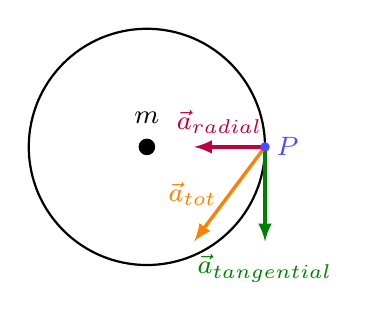
\begin{tikzpicture}
				[
				x=1cm, y=1cm, scale=0.6, font=\footnotesize, >=latex 
				%Voreinstellung für Pfeilspitzen
				]
				%Raster im Hintergrund
				%\draw[step=1, gray, very thin] (0,0) grid (5.5,5.5);
				\draw[thick] (0, 0) circle(2.5);
				\fill[black] (0, 0) circle(5pt) node [midway, above, yshift=7pt, scale=2] {$m$};
				\begin{scope}[xshift=2.5cm, yshift=0cm, rotate=0, scale=1]
					%Kräfte
					\draw [-latex, very thick, green!50!black] (0,0) -- ++(0,-2) node[below, scale=1.2] {$\vec{a}_{tangential}$};
					\draw [-latex, very thick, purple] (0,0) -- ++(-1.5,0) node[midway, above, scale=1.2, xshift=-3pt] {$\vec{a}_{radial}$};
					\draw [-latex, very thick, orange] (0,0) -- ++(-1.5,-2) node[midway, left, scale=1.2] {$\vec{a}_{tot}$};
					\fill [blue!70!white](0,0) circle (0.1) node[midway, right, scale=2] {$P$};;
				\end{scope}		
			\end{tikzpicture}
		\end{minipage}
		\hfill
		\begin{minipage}{0.55\linewidth}
			$a_{tangential} = \frac{dv}{dt} = \dot{v}$ \\
			\\
			$a_{radial} = \frac{v^2}{r}$ \\
			\\
			$ \boxed { F_{zentripetal} = m \, \frac{v^2}{r} }$ \\
			\\
			$ \boxed{ (F_{zentri})^2 + (F_{bremsen})^2 = (F_R)^2 }$
		\end{minipage}

		Wenn $a = 0 \Rightarrow F_{Zentri} = F_{Haft} $

	\subsection{Gleichförmige Bewegung $a_{tangential} = 0$}
	
		\begin{minipage}{0.6\linewidth}
			\textbf{tangential (Tacho)} \\
				\\
				$a_{tangential} = 0$ \\
				\\
				$v(t) = v_0 = \text{const}$ \\
				\\
				$s(t) = v_0 \cdot t + s_0$ \\
		\end{minipage}
		\hfill
		\begin{minipage}{0.35\linewidth}
			\textbf{radial} \\
				\\
				$a_{radial} = \frac{v^2}{r}$ \\
				\\
				\\
				\\
				\\
		\end{minipage}

	\subsection{Gleichm. beschl. Bewegung $a_{tangential} = \text{konst}$}		
		\begin{minipage}{0.45\linewidth}
			\textbf{tangential (Tacho)} \\
				\\
				$a_{tang} = a_0 = \text{const}$ \\
				\\
				$v(t) = a_{tang} \cdot t + v_0 $ \\
				\\
				$s(t) = \frac{1}{2} \, a_{tang} \cdot t^2 +  v_0 \cdot t + s_0$ \\
		\end{minipage}
		\hfill
		\begin{minipage}{0.5\linewidth}
			\textbf{radial} \\
				\\
				$a_{rad} = \frac{v^2}{r} = \omega^2r = (\alpha \cdot t)^2 \cdot r$\\
				\\
				\\
				\\
				\\
		\end{minipage}

		Die Gesamtbeschleunigung eines Systems $\vec{a}_{tot} = \vec{a}_{tangential} + \vec{a}_{radial} $ muss nicht zwingend konstant sein! Bei Änderungen der Richtung ändert die Gesamtbeschleunigung. 
	
	\subsection{Kreisbewegung}
		
		\subsubsection{Winkel $\phi$ (zurückgelegter Weg)}
		
		\begin{minipage}{0.5\linewidth}
			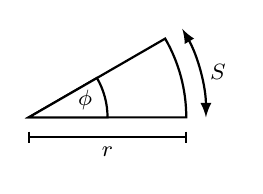
\begin{tikzpicture}
				[
				x=1cm, y=1cm, scale=1.0, font=\footnotesize, >=latex 
				%Voreinstellung für Pfeilspitzen
				]

				%Länge x Achse
				\draw [thick] (0,0) -- ++(2,0) node[below] {};
				\draw [thick] (1,0) node[below] {$r$};
				
				%Zahlen auf x-Achse
				\foreach \x in {0,2}
				\draw[shift={(\x,0)},color=black, thick] (0pt,2pt) -- (0pt,-2pt);
				
				%Winkelgugus
				\begin{scope}[xshift=0cm, yshift=0.25cm, rotate=0, scale=1]
					\filldraw[fill=white, thick] (0,0) -- (2,0) arc (0:30:2) -- cycle 
						node[midway, below, green!50!black, xshift=0pt, yshift=0pt] {};
					\filldraw[fill=white, thick] (0,0) -- (1,0) arc (0:30:1) -- cycle 
						node[midway, xshift=8pt, yshift=-1pt] {$\phi$};
				\end{scope}
				
				\draw [<->, thick] (2.25,0.25) arc (0:30:2.25) node[midway, right, xshift=0pt, yshift=0pt] {$S$};
			\end{tikzpicture}
		\end{minipage}
		\hfill
		\begin{minipage}{0.4\linewidth}
			$\boxed{ \text{Radiant: } \phi = \frac{s}{r} }$ 
		\end{minipage}

		\subsubsection{Winkelgeschwindigkeit $\omega= \frac{\phi}{t}$}
		
			$\omega := \lim \limits_{\Delta t \rightarrow 0} \frac{\phi(t + \Delta t) - \phi(t)}{\Delta t} = \frac{d \phi}{dt} = \dot{\phi}$ \\
			\\
			Der Betrag $v$ der (Bahn-) Geschwinndigkeit entspricht: $v = r \cdot \omega$ \\

			\begin{tabular}{ll}
				Umlaufzeit, Periode $T$ & Umlaufzeit für vollständige Umdrehung \\
				\\
				Drehzahl, Drehfrequenz $f$ & inverse Umlaufzeit   $f = \frac{1}{T}$ \\
				\\
				\\
			\end{tabular}
			
			\textbf{Wichtige Umrechnungsformeln} \\		 
				\\
				\boxed{
					\begin{tabular}{l c l l}
						$v = r \cdot \omega$ & $\Leftrightarrow$ & $\omega = \frac{v}{r}$ & \\		
						\\
						$f = \frac{1}{T}$ & $\Leftrightarrow$ & $T = \frac{1}{f}$ & \\
						\\
						$\omega = \frac{2 \, \pi}{T}$ & $\Leftrightarrow$ & $T = \frac{2 \, \pi}{f}$ & $\omega = \frac{2 \pi n}{60} $ \\
						\\
						$\omega = 2 \, \pi \, f$ & $\Leftrightarrow$ & $f = \frac{\omega}{2 \, \pi} $ & $v = \frac{\pi d n}{60} $ \\
					\end{tabular}
				}

		\subsubsection{Winkelbeschleunigung $\alpha = \frac{\omega}{t}$}
		
			$\alpha = \lim \limits_{\Delta t \rightarrow 0} \frac{\omega(t + \Delta t) - \omega(t)}{\Delta t} = \frac{d \omega}{dt} = \dot{\omega} = \frac{d^2 \, \phi}{d t^2} \ddot{\phi} $ \\
			\\
			$a_{tangential} = \frac{dv}{dt} = \frac{d}{dt} r \cdot \omega = r \cdot \alpha$

	\subsection{Gleichförmige Kreisbewegung}
		
		\begin{tabular}{l}
			$\alpha(t) = 0$ \\
			\\
			$\omega(t) = \omega_0 = \text{const}$ \\
			\\
			$\phi(t) = \omega_0 \, t + \phi_0$ 
		\end{tabular}

	\subsection{Gleichm. beschleunigte Kreisbewegung}
		
		\begin{tabular}{l}
			$\alpha(t) = \alpha_0 = \text{const} $ \\
			\\
			$\omega(t) = \alpha_0 \cdot t + \omega_0$ \\
			\\
			$\phi(t) = \frac{1}{2} \, \alpha_0 \cdot t^2 + \omega_0 \cdot t + \phi_0$ \\
		\end{tabular}

	\subsection{Senkrechter Wurf}

		\begin{minipage}{0.45\linewidth}
			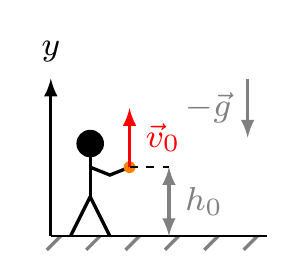
\begin{tikzpicture}
				[
				x=1cm, y=1cm, scale=0.5, font=\footnotesize, >=latex 
				%Voreinstellung für Pfeilspitzen
				]
				
				%Raster im Hintergrund
				%\draw[step=1, gray!50!white, very thin] (-2,-2) grid (5,5);
				
				%Zahlen auf x-Achse
				\foreach \x in {-0.75,0.25,1.25,2.25,3.25,4.25}
				\draw[shift={(\x,0)},color=gray, very thick] (0pt,0pt) -- (-10pt,-10pt);
				
				\draw [very thick] (0.5,0)--(0,1);
				\draw [very thick] (-0.5,0)--(0,1);
				\draw [very thick] (0,1)--++(0,1);
				\draw [very thick] (0,1.75)--(0.5,1.55)--(1,1.75);
				\fill (0,2.35) circle (0.35);
				\fill [orange](1,1.75) circle (0.15);

				%Länge x Achse
				\draw [thick] (-1,0) -- ++(5.5,0);
				\draw [-latex, very thick, red] (1,1.75)--++(0,1.5) node [midway, right, red, xshift=0pt, yshift=0pt, scale=1.5] {$\vec{v}_0$} {};
				\draw [-latex, very thick, gray] (4,4)--++(0,-1.5) node [midway, left, gray, xshift=0pt, yshift=0pt, scale=1.5] {$-\vec{g}$} {};
				\draw [-latex, very thick] (-1,0)--++(0,4) node [above, xshift=0pt, yshift=0pt, scale=1.5] {$y$} {};
				\draw [<->, very thick, gray] (2,0)--++(0,1.75) node [midway, right, gray, xshift=0pt, yshift=0pt, scale=1.5] {$h_0$} {};
				\draw [dashed, thick] (1,1.75)--++(1,0);
			\end{tikzpicture}
		\end{minipage}
		\hfill
		\begin{minipage}{0.5\linewidth}
			$a = -g = \text{const}$ \\
			\\
			$v(t) = -g \cdot t + v_0$ \\
			\\
			$h(t) = - \frac{1}{2} \, g \cdot t^2 + v_0 \cdot t + h_0$ \\
		\end{minipage}

		\subsubsection{Maximale Flughöhe $h_{max}$ bestimmen}
			Bei der maximalen Flughöhe $h_{max}$ gilt: $v(t) \overset{!}{=} 0$ \\
			\\
			$v_0 - g \cdot t_{max} \overset{!}{=} 0$ \qquad $\Rightarrow$ \qquad $t_{max} = \frac{v_0}{g}$ \\
			\\
			Nun wird $t_{max}$ in $h(t)$ eingesetzt: \\
			\\
			$h_{max} = h(t_{max}) = - \frac{g}{2} \, \frac{v_0^2}{g^2} + v_0 \, \frac{v_0}{g} + h_0 = \frac{v_0^2}{2 \, g} + h_0 $ \\
			\\
			\\
			\textbf{Hinweis: Die maximale Flughöhe kann auch über die potentielle und kinetische Energie berechnet werden!} \\
				$E_{kin} \overset{!}{=} 0 $ \qquad $E_{pot} \overset{!}{=} m \cdot g \cdot h_{max} $ \\
				$\frac{1}{2} \, m \cdot v^2 = m \cdot g \cdot h_{max}$ \quad $\Rightarrow$ \quad $h_{max} = \frac{m \, v^2}{2 \, m  \, g} =  \frac{v^2}{2 \, g} $  \\
				\\
				$\Rightarrow$ für \underline{abgeschlossene} Systeme!
	
	\subsection{Horizontaler Wurf}
	
		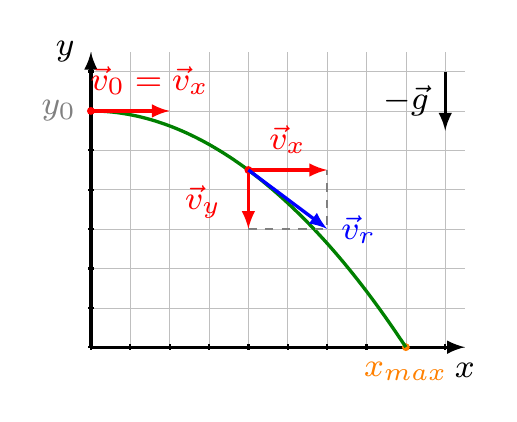
\begin{tikzpicture}
			[
			x=1cm, y=1cm, scale=0.5, font=\footnotesize, >=latex 
			%Voreinstellung für Pfeilspitzen
			]
			
			%Raster im Hintergrund
			\draw[,step=1, gray!50!white, very thin] (0,0) grid (9.5,7.5);
			
			%Länge x-Achse
			\draw [-latex, very thick] (0,0) -- ++(9.5,0) node[below, scale=1.5] {$x$};
			
			%Länge y-Achse
			\draw [-latex, very thick] (0,0) -- ++(0,7.5) node[left, scale=1.5] {$y$};
			
			%Zahlen auf y-Achse 
			\foreach \y in {0,1,2,3,4,5,6,7}
			\draw[shift={(0,\y)}, color=black, thick] (2pt,0pt) -- (-2pt,0pt);
			
			%Zahlen auf x-Achse
			\foreach \x in {0,1,2,3,4,5,6,7,8,9}
			\draw[shift={(\x,0)},color=black, thick] (0pt,2pt) -- (0pt,-2pt);
			
			\draw [] (0,6) node[gray, left, scale=1.5] {$y_{0}$};	
			\draw [] (8,0) node[orange, below, scale=1.5] {$x_{max}$};	
			\fill [orange] (8,0) circle (0.1);
			% die Parable halt
			\draw[green!50!black, very thick] (0,6) parabola bend (0,6) (8,0);			

			%Vektor v0
			\fill [red] (0,6) circle (0.1);
			\draw[-latex, very thick, red] (0,6) -- ++ (2,0) node [midway, above, red, xshift=7pt, yshift=0pt, scale=1.5] {$\vec{v}_0=\vec{v}_x$} node (v) {};		
			
			%Vektor v1
			\fill [red] (4,4.5) circle (0.1);
			\draw[-latex, very thick, red] (4,4.5) -- ++ (2,0) node [midway, above, red, xshift=0pt, yshift=0pt, scale=1.5] {$\vec{v}_x$} node (v) {};
			\draw[-latex, very thick, red] (4,4.5) -- ++ (0,-1.495) node [midway, left, red, xshift=-4pt, yshift=-1pt, scale=1.5] {$\vec{v}_y$} {};
			\draw[-latex, very thick, blue] (4,4.5) -- ++ (2,-1.495) node [midway, below, blue, xshift=0.9cm, yshift=0pt, scale=1.5] {$\vec{v}_r$} {};
			\draw [dashed, gray, thick] (4,3)--(6,3)--(6,4.5);
			
			\draw [-latex, very thick] (9,7)--(9,5.5) node [midway, left, xshift=0cm, yshift=0pt, scale=1.5] {$-\vec{g}$} {};
		\end{tikzpicture}

		Der horizontale Wurf muss komponentenweise beschrieben werden \\
		x-Achse: gleichförmige, unbeschleunigte Bewegung \\
		y-Achse: gleichmässig beschleunigte Bewegung \\
		
		\begin{minipage}{0.45\linewidth}
			\textbf{x-Achse} \\
				\\
				$a_x = 0$ \\
				$v_x = v_0$ \\
				$x = v_0 \cdot t + x_0$ \\
		\end{minipage}	
		\hfill	
		\begin{minipage}{0.45\linewidth}
			\textbf{y-Achse} \\
				\\
				$a_y = -g$ \\
				$v_y = -g \cdot t$ \\
				$y = - \frac{1}{2} \, g \cdot t^2 + y_0$ \\
		\end{minipage}	
		
		\textbf{Tipp:} Lege den Koordinatenursprung in den Abwurf-Ort
	
		\subsubsection{Beschreibung der Flugbahn (Eliminierung von $t$)}	
			Die y-Koordinate soll als Funktion der x-Koordinate ausgedrückt werden: $y = f(x)$ \\
			\\
			$x = v_0 \, t$ \quad $\Leftrightarrow$ \quad $t = \frac{x}{v_0}$ \quad $\Rightarrow$ \quad $y = - \frac{1}{2} \, g \cdot t^2 = - \frac{g}{2} \frac{x^2}{v_0^2} = y(x)$
			
	\subsection{Schiefer Wurf}
	
		\begin{tikzpicture}
			[
			x=1cm, y=1cm, scale=1.3, font=\footnotesize, >=latex 
			%Voreinstellung für Pfeilspitzen
			]
			
			%Raster im Hintergrund
			\draw[step=1, gray!50!white, very thin] (0,0) grid (4.5,1.5);
			
			%Länge x-Achse
			\draw [-latex] (0,0) -- ++(4.5,0) node[below] {$x$};
			
			%Länge y-Achse
			\draw [-latex] (0,0) -- ++(0,1.5) node[left] {$y$};
			
			%Zahlen auf y-Achse 
			\foreach \y in {0,1}
			\draw[shift={(0,\y)}] (2pt,0pt) -- (-2pt,0pt);
			
			%Zahlen auf x-Achse
			\foreach \x in {0,1,2,3,4}
			\draw[shift={(\x,0)},color=black] (0pt,2pt) -- (0pt,-2pt);
			
			\filldraw[fill=green!20!white, draw=green!50!black] (0,0) -- (0.75,0) arc (0:45:0.75) -- cycle node[midway, below, green!50!black, xshift=4pt, yshift=2pt] {$\phi$};
			
			%gestrichelte linie
			\draw [dashed, orange, thick] (2,0) -- (2,1);
			
			\draw [] (0,1) node[gray, left] {$h_{max}$};
			\draw [] (0,0) node[gray, left] {$h_{0}$};	
			\draw [] (0,0) node[orange, below] {$0$};
			\draw [] (4,0) node[orange, below] {$s_{max}$};	
			\draw [] (2,0) node[orange, below] {$\dfrac{s_{max}}{2}$};	
			
			% die Parable halt
			\draw[red,thick] (0,0) parabola bend (2,1) (4,0);
			
			\draw [dashed, gray, thick] (2,1)-- (0,1);		
			
			%Vektor v
			\draw[-latex, thick, blue] (0,0) -- (0.8,0.8) node [midway, above, blue, xshift=-4pt, yshift=-1pt] {$\vec{v}$} node (v) {};		
			
		\end{tikzpicture}

		Der schiefe Wurf muss komponentenweise beschrieben werden \\
		x-Achse: gleichförmige, unbeschleuigte Bewegung \\
		y-Achse: gleichmässig beschleunigte Bewegung \\
		
		\begin{minipage}{0.45\linewidth}
			\textbf{x-Achse} \\
				\\
				$a_x = 0$ \\
				$v_x = v_0 \cdot \cos(\phi)$ \\
				$x = v_0 \cdot \cos(\phi) \cdot t + x_0$ \\
		\end{minipage}	
		\hfill	
		\begin{minipage}{0.45\linewidth}
			\textbf{y-Achse} \\
				\\
				$a_y = -g$ \\
				$v_y = -g  \cdot t + v_0 \cdot \sin(\phi)$ \\
				$y = - \frac{1}{2} \, g \cdot t^2 + v_0 \cdot \sin(\phi) \cdot t + y_0$ \\
		\end{minipage}	
		
		\textbf{Tipp:} Lege den Koordinatenursprung in den Abwurf-Ort

		\subsubsection{Beschreibung der Flugbahn (Eliminierung von $t$)}	
			Die y-Koordinate soll als Funktion der x-Koordinate ausgedrückt werden: $y = f(x)$ \\
			\\
			$x(t) = v_0 \cdot \cos(\phi) \cdot t$ \quad $\Rightarrow$ \quad $t = \frac{x}{v_0 \cdot \cos(\phi)}$ \\
			\\
			$\Rightarrow$ \quad $y = - \frac{g}{2 \, v_0^2 \cdot \cos^2(\phi)} \cdot x^2 + \tan(\phi) \cdot x = y(x)$

		\subsubsection{Ansätze zur Bestimmung von Extrema}		
			\begin{tabular}{ll}
				max. Wuftweite $s_{max}$ & $y \overset{!}{=} 0 $ \quad ($\phi \in \{ 45° ; 135° \}$)\\
				& $s_{max} = x_{max} \in \{ 0, \frac{2 \, v_0^2}{g} \cos(\phi) \cdot \sin(\phi) \}$ \\
				\\
				Elevationswinkel & $\phi = \frac{1}{2} \arcsin \big( \frac{g \cdot d}{v_0^2} \big) = \frac{1}{2} \arcsin \big( \frac{g \cdot x_{max}}{v_0^2} \big)$ \\
				\\
				max. Wurfhöhe & $v_y \overset{!}{=} 0 $ \\
				& $x_{maxH"ohe} =  h_{max} = \frac{s_{max}}{2} = \frac{x_{max}}{2}$ \\
				& $y(x_{maxH"ohe}) = \frac{v_0^2 \cdot sin^2(\phi)}{2 \, g}$
			\end{tabular}
